

\documentclass[../../e3_tp2_main.tex]{subfiles}

\begin{document}

\section{Ejercicio 8}

Se propuso el diseño de un circuito que permita medir distancias utilizando un sensor ultrasónico de distancia (HC-SR04).\par 

El circuito debe cumplir con los siguientes requerimientos: 
\begin{itemize}  
\item \underline{\textit{trigger}}: pin de entrada que dispara la medición en el flanco positivo. 
\item \underline{\textit{trigger enable}}: pin de entrada que habilita la señal de disparo.
\item \underline{\textit{meas}}: 8 bits de salida que indican el tiempo medido en unidades de 100$\micro s$.
\item \underline{\textit{meas ready}}: pin de salida que indica que la medición ha finalizado. 
\end{itemize}

\subsection{Sensor HC-SR04}

El sensor de distancia HC-SR04\footnote{Datasheet del sensor: \url{https://www.mouser.com/ds/2/813/HCSR04-1022824.pdf} (consultado: 13/10/18).} es un sensor de distancia ultrasónico. Posee cuatro terminales: dos de alimentación ($V_{CC}$ y \textit{gnd}), el \textit{trigger} y \textit{echo}.
\par El terminal de \textit{trigger} acciona la medición. Para ello se debe cambiar el estado de este terminal a \textit{high} por más de 10$\micro s$ y, de esta manera, el sensor comienza a medir. Luego por el pin de \textit{echo} se devuelve un pulso de ancho T $\micro s$. La duraci\'on de este pulso es proporcional a  la distancia medida: Distancia = $ \frac {1\micro s}{58}[cm]$.
\par El rango de medición del sensor es de 2cm a 4 metros. Por ende, el ancho del pulso devuelto por \textit{echo} es de entre 116$\micro s$ y 23200$\micro s$.
\begin{figure}[H]	
	\centering
	\fbox{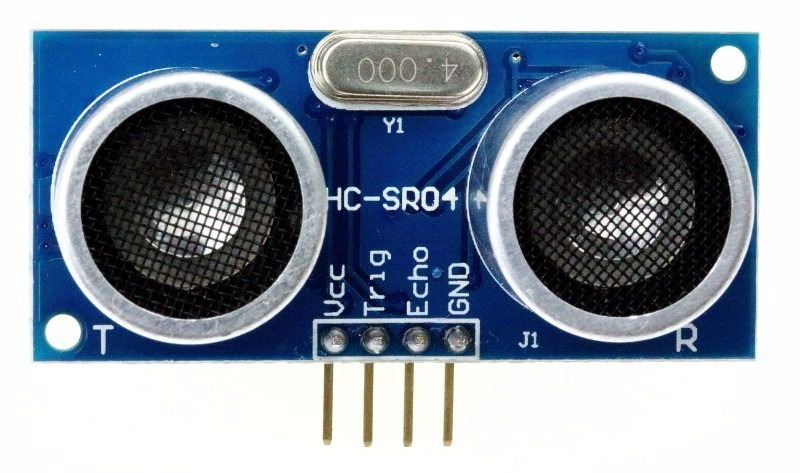
\includegraphics[width=0.4\textwidth]{imagenes/sensor.jpg}}
	\caption{Sensor de distancia}
\end{figure}

\begin{figure}[H]	
	\centering
	\fbox{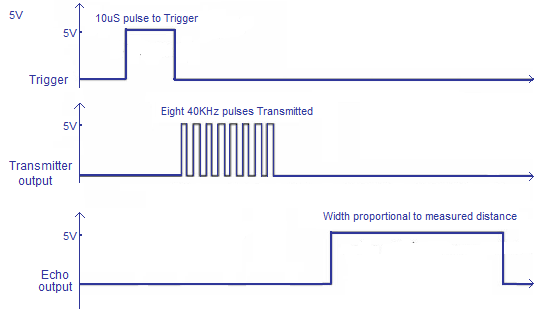
\includegraphics[width=0.45\textwidth]{imagenes/sensor_t.png}}
	\caption{Diagrama temporal}
\end{figure}

\subsection{Circuito Implementado}

Se modularizó el circuito de la siguiente manera:
\begin{figure}[H]	
	\centering
	\fbox{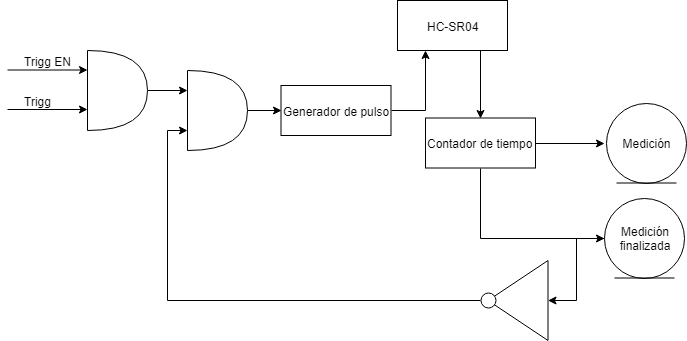
\includegraphics[width=0.45\textwidth]{imagenes/dBloques.png}}
	\caption{Diagrama de bloques}
	\label{fig:dBloques}
\end{figure}
Los dos módulos principales, tal como se muestra en la imagen \ref{fig:dBloques}, son el generador de pulso y el contador de tiempo.
\par El generador de pulso, cuando recibe un flanco positivo, genera un pulso mayor a 10$\micro s$ para que el sensor comience a medir.
\par El contador de tiempo, por otra parte, mide el ancho del pulso devuelto por \textit{echo} y lo devuelve en 8 bits. También se encarga de indicar que la medición finaliz\'o.

\subsubsection{Generador de pulso}
El generador de pulso se implementó con un LM555. El circuito utilizado fue el de la figura \ref{fig:555c}. Este circuito genera un pulso de ancho $t=R_a C \cdot1.1$s. Para generar el disparo se debe generar un pulso menor que el configurado.
\par Como el sensor requiere un ancho de pulso mayor de 10$\micro s$, se eligieron los componentes para un pulso de 50$\micro s$, por ende el capacitor $C=10$nF y $R_a=5k \Omega$

\begin{figure}[H]	
	\centering
	\fbox{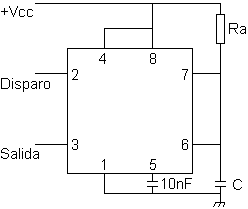
\includegraphics[width=0.3\textwidth]{imagenes/555C.png}}
	\caption{Circuito del generador de pulsos}
	\label{fig:555c}
\end{figure}
Para evitar que al generador de pulso le ingrese una señal mayor a 50$\micro s$ se le coloc\'o a la entrada (disparo) un RC con tiempo característico de 10$\micro s$. 

\subsubsection{Contador de tiempo}
Para medir cu\'anto tiempo el pulso de \textit{echo} est\'a en \textit{high}, se utilizó un contador de 8 bits y una señal cuadrada de 50\% de \textit{duty cycle} como \textit{clock}.
\par El contador utilizado cuenta flancos positivos de \textit{clock}. Por ende, para contar cu\'anto tiempo la señal de \textit{echo} estuvo en \textit{high}, se conectó la entrada de clock del contador, a la salida de una \textit{and}. Las entradas de la \textit{and} son la señal de \textit{echo} y una señal cuadrada de 10$kHz$. De esta manera, cada vez que ocurre un flanco de \textit{clock} y la señal echo esta en \textit{high} el contador incrementa en una unidad. Debido a que la frecuencia de la señal cuadrada es de 10$kHz$, cada unidad en el contador representa 100$\micro s$.
\begin{figure}[H]	
	\centering
	\fbox{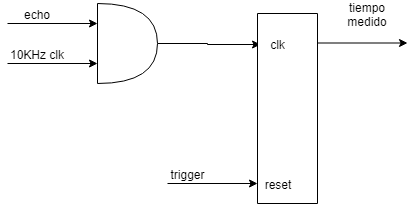
\includegraphics[width=0.4\textwidth]{imagenes/contador.png}}
	\caption{Contador de tiempo}
\end{figure}
\par En cuanto al reset del contador, se lo conect\'o al \textit{trigger} del sensor. De esta manera, cada vez que se dispara una medición el contador vuelve a cero.
\subsubsection{Meas ready}

En cuanto a la salida de \textit{meas ready}, bast\'o con negar la señal de \textit{echo}. Mientras no haya medición, la señal de \textit{echo} se mantiene en \textit{low} y por ende \textit{meas ready} se mantiene en high. Cuando \textit{echo} está en \textit{high}, en cambio, quiere decir que se está midiendo, y \textit{meas ready} se encuentra entonces en \textit{low}.

\subsubsection{Prototipo}
Previo al diseño final del circuito, se decidió construir un prototipo del mismo en una \textit{protoboard}, para así probar el correcto funcionamiento de cada etapa y del conjunto. 
\begin{figure}[H]	
	\centering
	\fbox{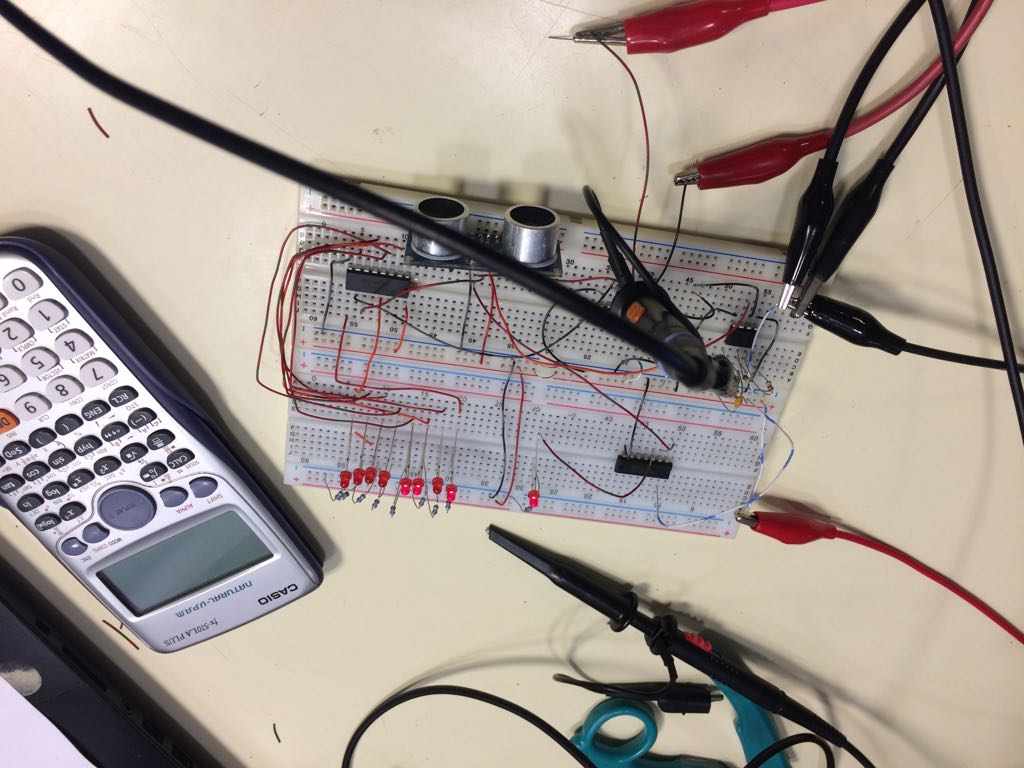
\includegraphics[angle=180,width=0.45\textwidth]{imagenes/prototipo.jpeg}}
	\caption{Prototipo del circuito}
\end{figure}
El prototipo funcion\'o correctamente, tal como se puede apreciar en \href{https://youtu.be/xzRgiA1r85w}{\underline{este video}}. Se procedió, pues, al armado de la placa.
\subsubsection{Circuito}

El circuito final construido posee las siguientes características:
\begin{itemize}
	\item Entrada de \textit{trigger}, \textit{trigger enable} y \textit{clock}. El \textit{clock} al que se lo debe conectar es de 10$kHz$ (señal cuadrada, 5V de amplitud y 50\% de \textit{duty cycle}).
	\item Salida 8 bits que indican el tiempo medido, y 1 bit que indica que la medición finaliz\'o.
\end{itemize}

\begin{figure}[H]	
	\centering
	\fbox{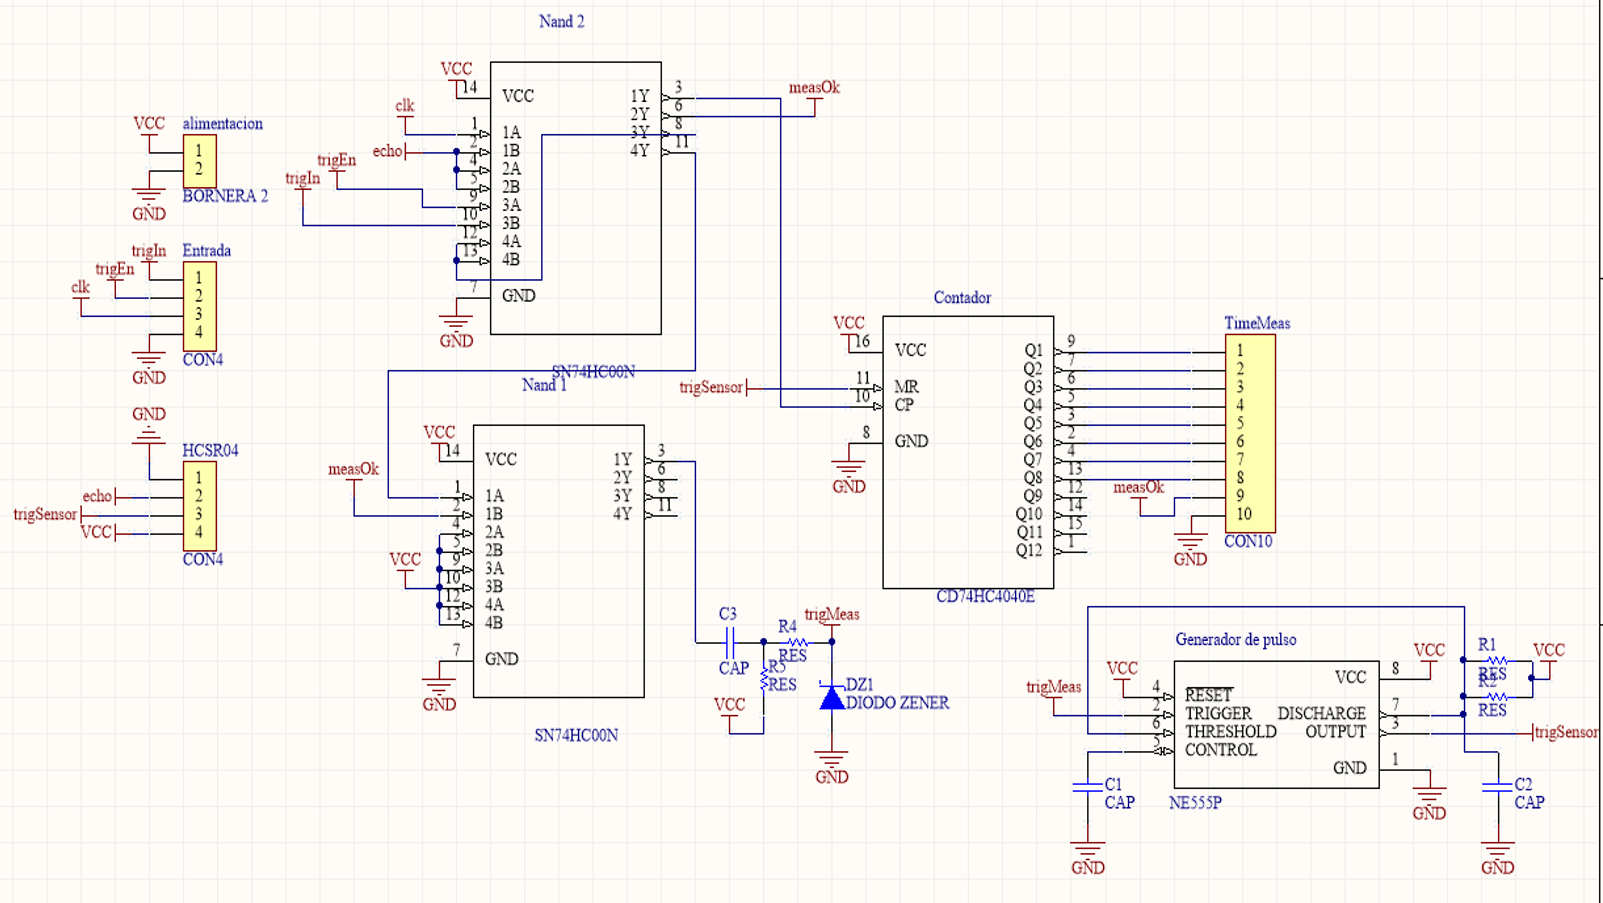
\includegraphics[width=0.45\textwidth]{imagenes/esquematico.png}}
	\caption{Esquem\'atico}
\end{figure}

\begin{figure}[H]	
	\centering
	\fbox{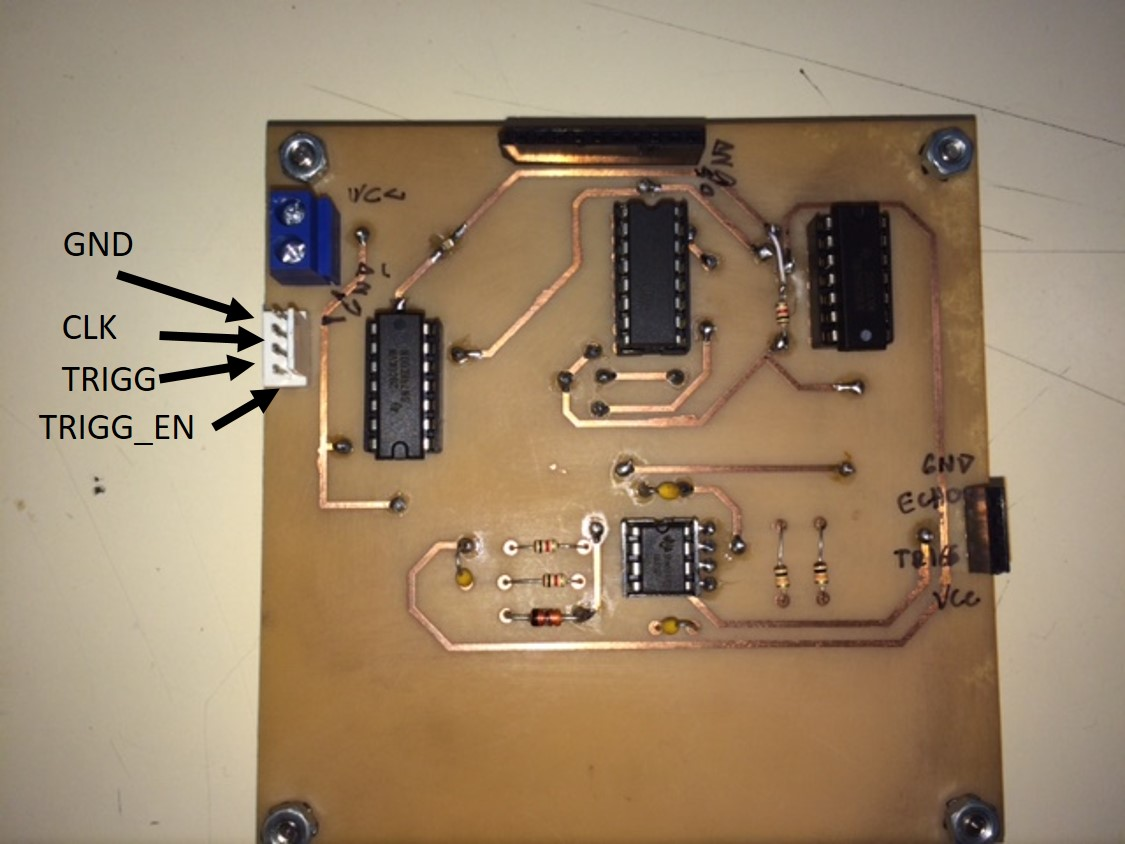
\includegraphics[width=0.45\textwidth]{imagenes/placa1.jpg}}
	\caption{PCB}
\end{figure}

\begin{figure}[H]	
	\centering
	\fbox{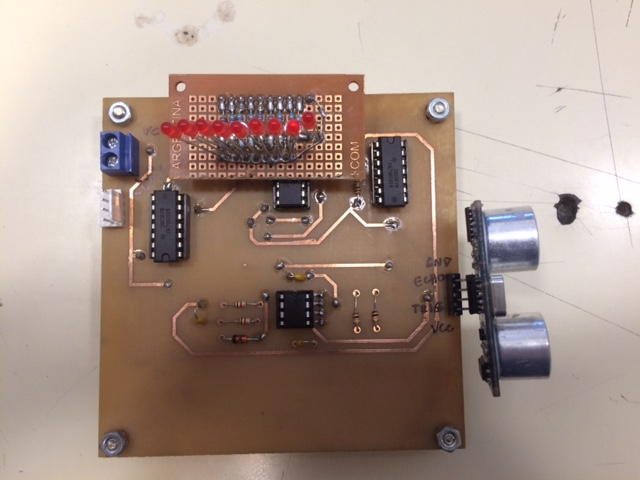
\includegraphics[width=0.45\textwidth]{imagenes/placa2.jpg}}
	\caption{PCB con sensor y led para indicar la salida}
\end{figure}

\subsubsection{Simulación}
Se simul\'o en Iverilog el circuito, y con GTKWave se visualizó su comportamiento en el tiempo.
\par Los módulos utilizados en la simulación son los mismos que los anteriormente descriptos, es decir hay un módulo encargado de generar un pulso y otro de contar el tiempo.\par

La figura \ref{fig:simg} es la simulación temporal del circuito. "meas" es el resultado de la medición, "sEcho" es el pulso devuelto por el sensor, "sTrigger" es el pulso que el circuito le envía al sensor para comenzar la medición, "trigger" es el pulso que recibe el circuito para comenzar a medir, y "meas ready" indica que la medición finaliz\'o.
\par Tal como se observa en la imagen, primero se dispara el \textit{trigger}, posteriormente el circuito genera en sTrigger un pulso de ancho 50$\micro s$. Despu\'es sEcho pasa a \textit{high} (comienza a medir el sensor) y \textit{meas ready} pasa a \textit{low}. El contador comienza a contar cu\'antos pulsos de \textit{clock} la señal de echo estuvo en \textit{high}. Cuando sEcho pasa a \textit{low} (la medición finaliz\'o) y \textit{meas ready} pasa a \textit{high}. Como el ancho del echo es de 500$\micro s$, el contador llegó a 5.

\begin{figure*}[t]	
	\centering
	\fbox{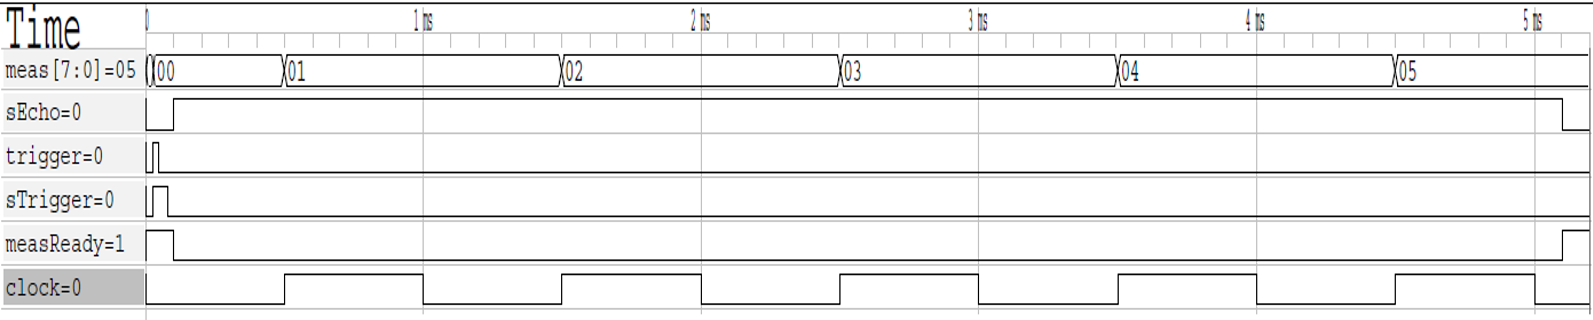
\includegraphics[width=0.9\textwidth]{imagenes/gtksim.png}}
	\caption{Simulación}\label{fig:simg}
\end{figure*}

\end{document}
